% 3_method.tex
\section{Method}
\label{sec:method}

\subsection{Problem Formulation}

In non-parametric skill systems, each skill $s$ has a Q-value $Q(s)$ that estimates its expected utility. When a task is executed using skill $s$, the standard Q-learning update is:
\begin{equation}
    Q_{\text{new}}(s) = Q_{\text{old}}(s) + \alpha (r_{\text{task}} - Q_{\text{old}}(s))
\end{equation}
where $r_{\text{task}} = 1$ if the task succeeded and $0$ otherwise, and $\alpha$ is the learning rate.

The contradiction arises because $r_{\text{task}}$ only captures task success, not content improvement. When a skill fails but refines its content (e.g., adding a new failure scenario to prevent the error), $r_{\text{task}} = 0$ and the Q-value decreases, even though the skill is now more knowledgeable.

\subsection{LQRL Update Rule}

We propose the LQRL update rule that decomposes the reward into task and learning components:
\begin{equation}
    Q_{\text{new}}(s) = Q_{\text{old}}(s) + \alpha \cdot [(1-\beta) \cdot r_{\text{task}} + \beta \cdot r_{\text{learning}}]
    \label{eq:lqrl}
\end{equation}
where $\beta \in [0, 1]$ is the layering weight and $r_{\text{learning}} \in [-0.5, 0.5]$ is the learning reward.

The learning reward $r_{\text{learning}}$ is evaluated by an LLM judge that compares the skill's content before and after the task:
\begin{itemize}
    \item $r_{\text{learning}} = +0.5$ if content improved (e.g., new failure scenario added)
    \item $r_{\text{learning}} = 0$ if content unchanged
    \item $r_{\text{learning}} = -0.5$ if content degraded (e.g., contradiction introduced)
\end{itemize}

When $\beta = 0$, \cref{eq:lqrl} reduces to standard Q-learning. When $\beta > 0$, failed tasks with content improvement can still receive positive Q-value updates.

\subsection{LLM-Based Content Evaluation}

The learning reward is computed by an LLM judge that analyzes whether the skill's content meaningfully improved. The evaluation considers:
\begin{enumerate}
    \item \textbf{Relevance}: Does the new content accurately describe the failure condition?
    \item \textbf{Actionability}: Can the new guidance help avoid similar failures?
    \item \textbf{Non-redundancy}: Does the new content add information beyond common sense?
    \item \textbf{Correctness}: Is the suggested solution valid?
\end{enumerate}

The judge returns a quality score $q \in [0, 0.5]$ that serves as $r_{\text{learning}}$. Low-quality content (below threshold $\tau = 0.1$) is not added to the skill.

\subsection{Failure Scenario Management}

When a task fails using skill $s$, the system constructs a \textit{failure scenario} describing the error pattern. Failure scenarios are stored in the skill with bounded storage:
\begin{itemize}
    \item Maximum 10 failure scenarios per skill
    \item Minimum quality threshold of 0.1 to accept new scenarios
    \item Merge similar scenarios with similarity $> 0.8$
\end{itemize}

\begin{figure}[t]
    \centering
    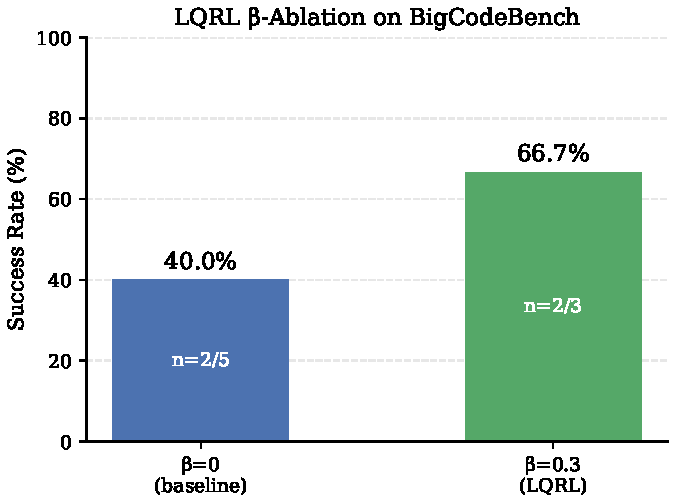
\includegraphics[width=0.48\textwidth]{figures/fig2_ablation.pdf}
    \caption{BigCodeBench success rate for baseline ($\beta=0$) versus LQRL ($\beta=0.3$).}
    \label{fig:ablation}
\end{figure}
